\chapter{Cosmology Lecture 1: Newtonian Cosmology and the First Friedmann Equation}

Cosmology is ancient, but the lecture begins by insisting that the science of cosmology is new. The modern subject starts when the universe is treated not as a cabinet of strange astronomical specimens, but as a physical system governed by equations. These notes follow Leonard Susskind's first cosmology lecture closely, and where the blackboard itself carries part of the argument, preserved board frames supplied through LazyingArt LLC and Video2Book are kept nearby as documentary evidence.

\section{From Ancient Cosmology to Modern Physics}

The opening move is a contraction of scale, not of the universe, but of the history we need. We do not begin with Greek speculation. We begin when cosmology becomes quantitative enough to be physics: first the discovery that the universe is expanding, and then the much later realization that the universe can be studied as a system with accurate equations tied to observation.

This is the real thesis of the lecture. The universe is to be studied the way we study any other physical system. It has matter, motion, density, and dynamics. It is not merely a catalogue of curious galaxies and peculiar stars. Once that point is accepted, the next question is immediate: what observations are stable enough to serve as the starting point?

The answer is not yet a dynamical law. We first ask what the universe looks like on large scales. Only after that do we decide how to describe it mathematically.

\section{Isotropy, Homogeneity, and the Cosmological Principle}

The lecture begins with an observational statement: on sufficiently large scales the universe looks approximately the same in every direction. This is what we mean by isotropy. One must average over enough sky, and one must look far enough away that the local clutter of our own galaxy no longer dominates the view. But after that averaging, the large-scale sky looks remarkably uniform.

Homogeneity is a different statement. It does not mean the same in every direction. It means the same from place to place. If we were to move far away and look around from another galaxy, we would again see essentially the same sort of large-scale universe.

In the early part of the lecture Susskind is content to treat galaxies as particles. That is exactly the right level of description for what follows. The individual internal structure of a galaxy is irrelevant here. What matters is that matter is distributed through space, and that on large enough scales this distribution is approximately uniform.

That large-scale uniformity is only approximate. The lecture is careful about this. There are clusters and superclusters; the universe is not literally featureless. But if we average over a sufficiently large region, the irregularities are smoothed out and the large-scale description becomes homogeneous.

This is the cosmological principle: on sufficiently large scales the universe is approximately homogeneous and isotropic.

\subsection{Question \& Answer}

\paragraph{Question.} Why should isotropy around us suggest homogeneity rather than merely indicating that we happen to sit at some special central location?

\paragraph{Answer.} The lecture's answer is geometric and deliberately simple. If the universe were isotropic around us but not homogeneous, then the only way to arrange that would be something shell-like: matter distributed in a way that is rotationally symmetric about our position, but not the same from place to place. Yet if that were the true arrangement, then an observer who moved away from our location would no longer see an isotropic universe. Thus isotropy around us is compatible with inhomogeneity only if we occupy a very special position near the center of a specially arranged universe.

The lecture refuses that special pleading. Unless we believe that our location is distinguished in this way, isotropy strongly suggests homogeneity. This is the real motivation for the cosmological principle in the lecture: not dogma, but the refusal to put ourselves at a miraculous center.

Later cosmology would bring stronger evidence, especially from the cosmic microwave background. But the lecture wants the logic first. The principle was historically used before it was firmly established, and then the observations gradually justified it.

\section{Freeze the Galaxies into a Grid}

Once the large-scale universe is taken to be homogeneous, the next step is to choose coordinates. Here the lecture makes a very characteristic move: choose them cleverly.

We introduce coordinates \(x,y,z\), but they are not physical lengths measured in meters. They are labels on a grid. And the smart choice is to let that grid move with the galaxies, so that each galaxy always sits at a fixed coordinate position. The galaxies are then frozen into the coordinate lattice, while the lattice itself may expand or contract.

This would be impossible if the large-scale motion were random. If different nearby galaxies wandered in unrelated directions, there would be no coherent grid to attach coordinates to. But that is not what the observations suggest. On large scales the galaxies move coherently, as if embedded in a common expanding structure. That observation is what motivates comoving coordinates.

If two galaxies \(A\) and \(B\) are separated only in the \(x\)-direction, we write their physical distance as
\begin{equation}
d_{AB}=a(t)\,\Delta x_{AB}.
\end{equation}
More generally, for arbitrary separation on the grid,
\begin{equation}
d_{AB}=a(t)\sqrt{(\Delta x)^2+(\Delta y)^2+(\Delta z)^2}.
\end{equation}
The single function \(a(t)\) is the scale factor. It contains all the time dependence. The coordinate separations are fixed; the physical distances change only because the scale factor changes.

Now differentiate. Since the galaxies are fixed on the grid, the coordinate separations do not change with time. Therefore
\begin{align}
v_{AB}&=\frac{d}{dt}d_{AB}=\dot a(t)\,\Delta x_{AB},\\
\frac{v_{AB}}{d_{AB}}&=\frac{\dot a}{a}\equiv H(t),\\
v_{AB}&=H(t)\,d_{AB}.
\end{align}
This is Hubble's law, now derived as the natural kinematics of a frozen grid whose scale changes with time.

The lecture pauses over the terminology. The Hubble constant is not really constant in time. What is constant is that, at a given time, the ratio \(v/d\) is the same everywhere. The more accurate phrase is Hubble parameter:
\begin{equation}
H(t)=\frac{\dot a}{a}.
\end{equation}

The lecture later reminds us that this is a large-scale statement. Bound systems can have peculiar motion on top of the average expansion. The law is not meant to describe the motion of every nearby galaxy pair in detail; it is the averaged kinematics of the homogeneous universe.

\subsection{Question \& Answer}

\paragraph{Question.} Are we not very nearly assuming Hubble's law when we write all distances as one common function \(a(t)\) times fixed coordinate separations?

\paragraph{Answer.} The lecture answers this directly: yes, the connection is close. We would not have guessed this ansatz in complete ignorance. Hubble's discovery is part of the reason for writing distances this way. But the point of the construction is not to pretend otherwise. The point is to reinterpret the observed recession law in a geometrically useful form. Instead of treating every galaxy pair separately, we describe all relative motion through one scale factor. What looked like many different velocities becomes one coherent motion of the grid itself.

That is already a gain. It turns an empirical regularity into a coordinate framework within which dynamics can later be written.

\section{Mass in a Comoving Cell}

Before Newton enters, the lecture takes a bookkeeping detour. It is calm and essential.

Take a coordinate cell of size \(\Delta x\,\Delta y\,\Delta z\), large enough that small-scale clumpiness has been averaged over. The mass in that coordinate cell is proportional to its coordinate volume, so we write
\begin{equation}
m_{\text{cell}}=\nu\,\Delta x\,\Delta y\,\Delta z,
\end{equation}
where \(\nu\) is the mass per unit coordinate volume.

Now ask for the physical volume of the same cell. Each coordinate edge is multiplied by the scale factor, so the physical volume is
\begin{equation}
V_{\text{cell}}=a^3\,\Delta x\,\Delta y\,\Delta z.
\end{equation}
Therefore the physical density is
\begin{equation}
\rho=\frac{m_{\text{cell}}}{V_{\text{cell}}}=\frac{\nu}{a^3}.
\end{equation}

This is exactly what one expects. If the universe expands, the same comoving mass occupies a larger physical volume and the density decreases. If the universe contracts, the density increases.

The lecture emphasizes the meaning of \(\nu\). It is constant because the galaxies move with the grid. A comoving cell keeps the same galaxies inside it, so it keeps the same mass. At this point nothing dynamical has happened. We have only chosen coordinates and kept track of how mass density transforms as the grid expands.

\section{Newton at the Center}

Now enters Newton.

Susskind makes the transition theatrically, and the notes should preserve that rhythm. Up to this point Euclid could have done the geometry. Now we ask for forces and accelerations.

Choose an origin. The lecture chooses it where Newton, naturally enough, places himself: at the center. That choice is not a physical privilege; it is a calculational convenience. The final equation must not depend on which galaxy we call the origin.

Let a representative galaxy have fixed comoving radius
\begin{equation}
R=\sqrt{x^2+y^2+z^2}.
\end{equation}
Its physical distance from the chosen origin is
\begin{equation}
d=a(t)R.
\end{equation}
Since \(R\) is fixed for that galaxy,
\begin{equation}
v=\dot a\,R,\qquad \text{acceleration}=\ddot a\,R.
\end{equation}

The crucial ingredient is Newton's theorem. In an isotropic situation, the gravitational effect of all matter outside the sphere through the galaxy cancels, while all the matter inside may be treated as if concentrated at the center.

\begin{figure}[t]
\centering

\includegraphics[width=0.82\textwidth]{lecture_01_figure_04.png}
\caption{The Newtonian side of the lecture: inverse-square force law and radial particle sketch. The distance symbol on the board is not notationally stable, so we standardize the derivation below in terms of \(d=aR\).}
\end{figure}

\begin{figure}[t]
\centering
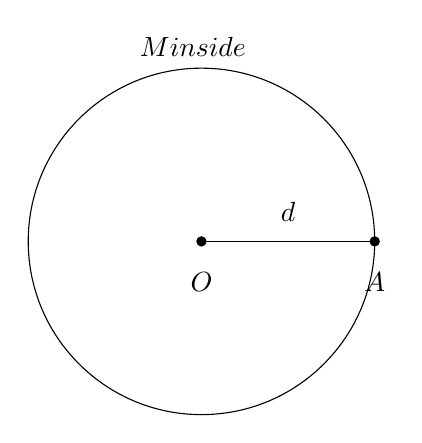
\begin{tikzpicture}[scale=1.1]
\draw (0,0) circle (2);
\fill (0,0) circle (0.06);
\draw (0,0) -- (2,0);
\fill (2,0) circle (0.06);
\draw (1,0.12) node[above] {\(d\)};
\draw (0,-0.25) node[below] {\(O\)};
\draw (2,-0.25) node[below] {\(A\)};
\draw (-0.1,2.25) node {\(M \text{ inside}\)};
\end{tikzpicture}
\caption{Clean version of the Newtonian reduction used in the lecture: a representative galaxy \(A\) lies on a sphere of radius \(d\), and only the mass inside that sphere contributes to its gravitational acceleration.}
\end{figure}

Let \(M\) be the mass inside the sphere of radius \(d\). Then
\begin{equation}
M=\frac{4\pi}{3}\rho\,d^3.
\end{equation}
The Newtonian inward acceleration of the galaxy is
\begin{equation}
-\frac{GM}{d^2}.
\end{equation}
Equating this to the kinematic acceleration \(\ddot a\,R\), we obtain
\begin{equation}
\ddot a\,R=-\frac{GM}{d^2}.
\end{equation}
Now substitute \(d=aR\) and \(M=\frac{4\pi}{3}\rho d^3\):
\begin{align}
\ddot a\,R
&=-\frac{G}{d^2}\left(\frac{4\pi}{3}\rho\,d^3\right)\nonumber\\
&=-\frac{4\pi G}{3}\rho\,d\nonumber\\
&=-\frac{4\pi G}{3}\rho\,aR.
\end{align}
Divide by \(aR\), and the representative galaxy label drops out:
\begin{equation}
\frac{\ddot a}{a}=-\frac{4\pi G}{3}\rho.
\end{equation}
This is the first central dynamical equation of the lecture. It is universal: it holds for every representative galaxy because the dependence on \(R\) has disappeared.

Substituting \(\rho=\nu/a^3\) gives the form that also appears on the board,
\begin{equation}
\frac{\ddot a}{a}=-\frac{4\pi G\nu}{3a^3}.
\end{equation}

\begin{figure}[t]
\centering

\includegraphics[width=0.88\textwidth]{lecture_01_figure_03.png}
\caption{Board state joining the boxed acceleration equations to the Newtonian one-particle analogy. The lecture moves back and forth between these two pictures rather than treating them as separate subjects.}
\end{figure}

A useful corollary is immediate. If \(\rho\neq 0\), then the right-hand side is negative, so a homogeneous matter-filled universe cannot be static. Static means \(a(t)\) constant, hence \(\ddot a=0\). But the equation shows that \(\ddot a=0\) is possible only if \(\rho=0\). A filled universe cannot merely sit there.

\subsection{Question \& Answer}

\paragraph{Question.} If every place sees matter on both sides, why is the universe not static?

\paragraph{Answer.} The naive argument is appealing but wrong. It imagines that matter on one side is simply balanced by matter on the other side. Newton's theorem shows that the bookkeeping must be done differently. For a given representative galaxy, all the matter outside the sphere through that galaxy contributes no net force. What remains is the mass inside the sphere, and that mass acts as though concentrated at the center. The galaxy therefore feels an inward relative acceleration determined by the enclosed density.

This also clarifies why the homogeneity assumption matters so much. The enclosed mass must be proportional to the volume in the same way everywhere. That is what makes the resulting equation universal and independent of which galaxy we chose.

The lecture also addresses the arbitrariness of the origin. One may worry that if we pick a different origin, the force seems to point toward a different place. But once the transformation to the new frame is done carefully, including the inertial terms associated with the moving frame, the same universal equation for \(a(t)\) emerges. The final result does not privilege any galaxy.

\section{Acceleration Is Not Velocity}

At this point the lecture stops a common mistake before it can harden into intuition. The equation
\begin{equation}
\frac{\ddot a}{a}=-\frac{4\pi G}{3}\rho
\end{equation}
tells us that the acceleration is negative. It does \emph{not} tell us whether the universe is presently expanding or contracting. That is a statement about \(\dot a\), not about \(\ddot a\).

To make that distinction sharp, the lecture temporarily leaves cosmology and studies a much simpler problem: a particle moving in the gravitational field of the Earth.

\begin{figure}[t]
\centering

\includegraphics[width=0.78\textwidth]{lecture_01_figure_02.png}
\caption{Sparse board state at the start of the energy discussion. The lecture has written only the moving particle and its kinetic term; the missing potential term is exactly the question being raised.}
\end{figure}

Let \(x\) now denote the distance of the particle from the Earth. This \(x\) is not the earlier comoving coordinate. The particle satisfies the Newtonian equation
\begin{equation}
\ddot x=-\frac{GM}{x^2}.
\end{equation}
The minus sign tells us only that the acceleration points inward. It does not tell us the sign of the velocity. The particle may be moving outward with positive velocity and negative acceleration, in which case it is slowing down; or it may already be moving inward, in which case the same negative acceleration makes it fall faster.

\subsection{Question \& Answer}

\paragraph{Question.} Does \(\ddot a<0\) mean that the universe is contracting?

\paragraph{Answer.} No. It means that whatever \(\dot a\) is doing, it is being pushed downward. If \(\dot a>0\), the universe is expanding but slowing down. If \(\dot a<0\), the universe is contracting and the contraction is speeding up.

This is ordinary mechanics. A car can move forward while its acceleration is negative; the negative acceleration means braking, not backward motion. The lecture makes exactly this point in more concrete language. The same distinction applies to cosmology. A negative \(\ddot a\) is a deceleration law, not yet a verdict on the sign of \(\dot a\).

To decide whether an outward-moving particle turns around, one needs more than the force law. One needs energy.

For the Earth problem, the conserved energy is
\begin{equation}
E=\frac12 mv^2-\frac{GMm}{x}.
\end{equation}
This is the more useful equation for classifying the motion. If \(E<0\), the particle is bound and may turn around. If \(E>0\), it has beaten escape velocity and will not return. The edge case is
\begin{equation}
E=0.
\end{equation}
Setting \(E=0\) gives the escape velocity:
\begin{align}
\frac12 v^2&=\frac{GM}{x},\\
v_{\mathrm{esc}}^2&=\frac{2GM}{x}.
\end{align}

The lecture now transfers this entire classification to cosmology. A universe may be below escape velocity, above escape velocity, or exactly at the edge. The acceleration equation alone did not tell us which case we were in. Energy will.

\section{Zero Total Energy, Friedmann's Equation, and the \(t^{2/3}\) Law}

We now return to the representative galaxy at comoving radius \(R\). For all practical purposes, it is moving in the gravitational field of a point mass \(M\) at the center, where \(M\) is the mass enclosed by the comoving sphere through the galaxy. Because matter moves with the grid, that enclosed mass stays fixed:
\begin{equation}
M=\frac{4\pi}{3}\rho\,a^3R^3=\frac{4\pi}{3}\nu R^3.
\end{equation}
This is why the Earth analogy can be lifted almost intact into cosmology.

\begin{figure}[t]
\centering

\includegraphics[width=0.82\textwidth]{lecture_01_figure_05.png}
\caption{Board transition from kinetic to potential energy for the cosmological particle problem. The denominator of the potential term is not fully visible on the board, so the clean formula below follows the lecture's surrounding algebra.}
\end{figure}

The kinetic energy of the representative galaxy is
\begin{equation}
\frac12 m\dot a^{\,2}R^2,
\end{equation}
because its physical velocity is \(v=\dot a\,R\). The potential energy is
\begin{equation}
-\frac{GMm}{aR}.
\end{equation}
Therefore
\begin{equation}
E=\frac12 m\dot a^{\,2}R^2-\frac{GMm}{aR}.
\end{equation}
The lecture now specializes to the zero-energy case, the analog of exactly escape velocity:
\begin{equation}
E=0.
\end{equation}
Cancel the test mass \(m\), multiply by \(2\), and divide by \(a^2R^2\):
\begin{align}
0&=\frac12 \dot a^{\,2}R^2-\frac{GM}{aR},\\
\left(\frac{\dot a}{a}\right)^2&=\frac{2GM}{a^3R^3}.
\end{align}
Now introduce the physical volume of the sphere,
\begin{equation}
V=\frac{4\pi}{3}a^3R^3,
\end{equation}
and write
\begin{equation}
\frac{M}{V}=\rho.
\end{equation}
Then
\begin{equation}
\left(\frac{\dot a}{a}\right)^2
=\frac{8\pi G}{3}\rho.
\end{equation}
This is the Friedmann equation in the matter-only, zero-energy case.

The lecture stresses that this equation is more useful than the acceleration equation, even though it encodes the same physics for the special case under discussion. It is the cosmological version of the fact that Newton's second law and energy conservation are equivalent descriptions of the same mechanics.

Substituting \(\rho=\nu/a^3\) gives
\begin{equation}
\left(\frac{\dot a}{a}\right)^2=\frac{8\pi G\nu}{3a^3}.
\end{equation}
Since \(\nu\) is merely the mass per unit coordinate volume, its normalization is partly a matter of coordinate choice. The lecture therefore strips the equation to its essential form by absorbing the positive constant into the units:
\begin{equation}
\left(\frac{\dot a}{a}\right)^2=\frac{1}{a^3}.
\end{equation}

\begin{figure}[t]
\centering

\includegraphics[width=0.74\textwidth]{lecture_01_figure_06.png}
\caption{Matter-dominated Friedmann scaling on the board: first with its constants, then in normalized form. This is the algebraic basis for the statement that the expansion slows but does not turn around.}
\end{figure}

Now comes a qualitative payoff before the explicit solution. The right-hand side is always positive for any finite \(a\). Therefore \(H^2=(\dot a/a)^2\) never reaches zero. A turnaround would require \(\dot a=0\). But if \(\dot a\) were ever zero, then \(H^2\) would vanish, which this equation forbids for finite \(a\).

So the zero-energy universe slows down, but it never stops. It gets tired, but not tired enough to turn around.

To solve the equation, the lecture looks for a power-law solution:
\begin{equation}
a(t)=Ct^p.
\end{equation}
Then
\begin{align}
\dot a&=Cp\,t^{p-1},\\
\frac{\dot a}{a}&=\frac{p}{t},\\
\frac{1}{a^3}&=\frac{1}{C^3 t^{3p}}.
\end{align}
Substitute into the normalized Friedmann equation:
\begin{equation}
\frac{p^2}{t^2}=\frac{1}{C^3 t^{3p}}.
\end{equation}
Matching powers of \(t\) gives
\begin{equation}
3p=2,
\end{equation}
so
\begin{equation}
p=\frac23.
\end{equation}
Matching coefficients then determines the constant \(C\) in terms of the chosen normalization, but the lecture rightly emphasizes that the exponent is the important part. Thus
\begin{equation}
a(t)\propto t^{2/3}.
\end{equation}

This is the expansion law of the Newtonian matter-dominated universe at the critical escape velocity.

The lecture ends by reopening the problem. If the total energy is not zero, one must add another term. As a preview only, the next step has the form
\begin{equation}
\left(\frac{\dot a}{a}\right)^2=\frac{8\pi G}{3}\rho+\frac{C}{a^2},
\end{equation}
where this new \(C\) records the memory of the total energy and is unrelated to the amplitude \(C\) in the trial solution above. Positive total energy means no re-collapse; negative total energy means eventual turnaround and contraction.

Finally there is the modern correction. The simple Newtonian matter-only universe is decelerating. The real universe, at late times, accelerates. So this lecture gives us a model that is both powerful and incomplete: powerful because it contains the core logic of cosmological expansion, incomplete because the real universe contains more than pressureless matter.

\section{Summary}

The lecture unfolds in a very disciplined order. We begin with large-scale observations, use isotropy to motivate homogeneity, and adopt the cosmological principle as an averaged description of the universe. We then choose comoving coordinates so that galaxies are frozen into a moving grid, and from that single idea the scale factor \(a(t)\) and Hubble's law emerge kinematically.

Only after this does Newton enter. Newton's theorem reduces the many-body problem to the mass enclosed within a sphere, and this yields the universal acceleration equation
\begin{equation}
\frac{\ddot a}{a}=-\frac{4\pi G}{3}\rho.
\end{equation}
The Earth-projectile analogy then supplies the missing intuition: negative acceleration does not by itself tell us whether motion is outward or inward; energy decides whether turnaround occurs.

In the zero-energy case, energy conservation gives the Friedmann equation
\begin{equation}
\left(\frac{\dot a}{a}\right)^2=\frac{8\pi G}{3}\rho,
\end{equation}
and with \(\rho=\nu/a^3\) this leads to the matter-dominated law
\begin{equation}
a(t)\propto t^{2/3}.
\end{equation}
That is the lecture's first complete model of the universe: homogeneous, matter-dominated, decelerating, and exactly at the edge between re-collapse and eternal expansion. The extra terms needed for the real accelerating universe are the business of the next step.